\documentclass[a4paper]{report}

\usepackage[french]{babel}
\usepackage[T1]{fontenc}
\usepackage[utf8]{inputenc}
\usepackage{amsmath}
\usepackage{graphicx}	
\usepackage{soul}
\usepackage{ulem}
\usepackage{titlesec}
\usepackage{sectsty}
\usepackage{color}
\usepackage[top=1.25in, bottom=1.25in, left=1in, right=1in]{geometry}
\usepackage[colorinlistoftodos]{todonotes}
\usepackage{url}

\renewcommand{\thesection}{\Roman{section}}

\newcommand{\HRule}{\rule{\linewidth}{0.5mm}}


\begin{document}

%Images en-tête
\begin{figure}[htbp]
\begin{minipage}[c]{.45\linewidth}
\begin{flushright}

\includegraphics[width=6cm]{Bordeaux.png}\end{flushright}
\end{minipage}
\hfill
\begin{minipage}[c]{.45\linewidth}
\begin{flushleft}

\includegraphics[width=6cm]{MaBioVis.jpg}
\end{flushleft}
\end{minipage}
\end{figure}

%titre
\begin{center}
\LARGE{Cahier des charges} \\

\HRule \\[0.4cm]{
\huge\bfseries Outil d'interrogation SQL-Analyses statistiques \\ [0.4cm]
}
\HRule \\[2cm]

%Images

\begin{figure}[htbp]
\begin{minipage}[c]{.45\linewidth}
\begin{flushright}

\includegraphics[width=5cm]{latex.png}\end{flushright}
\end{minipage}
\hfill
\begin{minipage}[c]{.45\linewidth}
\begin{flushleft}

\includegraphics[width=6cm]{python.jpg}
\end{flushleft}
\end{minipage}
\end{figure}
\begin{center}

\includegraphics[width=4cm]{sql.png}
\end{center}

%Auteurs

\begin{minipage}{0.4\textwidth}
\begin{flushleft} \large
\emph{Concepteurs du projet} :\\
\vspace{1\baselineskip}
        Amal \textsc{Dahmani}\\
        Kevin \textsc{Jamart}\\
        Khaoula \textsc{Jlassi}\\
        Myriam \textsc{Lopez}\\
\end{flushleft}
\end{minipage}
\begin{minipage}{0.4\textwidth}
\begin{flushright} \large
\emph{Client} : Joris \textsc{Sansen}\\
\end{flushright}
\end{minipage}

\begin{center}

\large
Master 1 - \textsc{Bioinformatique} \\
Promotion 2014-2015

\end{center}

\end{center}

\newpage


%Sommaire
\tableofcontents

\newpage
\addcontentsline{toc}{section}{Introduction}


%Intro
\section*{Introduction}

Le LAboratoire Bordelais de Recherche en Informatique (LABRI)\cite{ref0} est une unité de recherche composée de 6 équipes dont Modèles et Algorithmes  pour la BioInformatique et la Visualisation d'Informations (MABioVis)\cite{ref1}.
 Cette équipe est subdivisée en deux thèmes dont EVADOME\cite{ref2}, dirigé par R. Bourqui qui travaille sur l'Exploration Visuelle et Analytique de Données Massives.\\
 Dans le cadre de leurs recherches, ils se sont notamment intéressés à examiner l'influence de l'encodage visuel des arêtes grâce à une évaluation de différentes représentations de graphes.\\

Lors de cette évaluation, plusieurs personnes ont effectué un exercice de recherche de chemins sur les différents dessins de graphes et certains paramètres mesurés afin de tester leurs performances.
 Ces différentes mesures ont été sauvegardées dans une base de données SQL et divers traitements sont effectués, notamment les calculs de moyennes, écart-type, tests statistiques et génération de graphiques.
 Ces traitements sont pour l’heure effectués grâce à un script Perl qui permet de récupérer les données requises dans la base de données et les transfère au logiciel de statistiques R.
 Finalement, il crée un compte-rendu des résultats obtenus dans un fichier \LaTeX et génère un fichier PDF.\\
 \\

Cependant, ce programme Perl est strictement adapté à l'unique base de donnée utilisée jusqu'à présent.
De plus, l'écriture du programme présente un manque de modularité, ce qui rend sa relecture ou modification difficile. 
Enfin, le script ne bénéficie pas d'interface graphique ce qui rend son utilisation austère et malaisée.\\

Au sein de ce projet nous allons proposer un outil qui reprendra les fonctionnalités actuelles du programme Perl, en améliorant son utilisation et sa prise en main (réparation/modification).\\

Dans le cadre de ce projet nous allons tâcher de proposer une interface graphique agréable et ergonomique dans le but d'accélérer et de faciliter l'étude et la manipulation de bases de données SQL.


\section{Etat de l'art}

Les langages les plus utilisés en bioinformatique\cite{ref3} sont : C, C++, C\#, Java, Perl et Python. C++, C\# et Java sont des langages de programmation orientés objet mais C est plutôt connu pour sa difficulté de prise en main et de manipulation.\\

Python\cite{refpyt} est un langage interprété. Perl\cite{refperl} et Python reposent pour une grande partie sur des bibliothèques riches et développées. Soutenus tous les deux par des communautés importantes, par conséquent, une documentation est disponible.\\
Bien que que Perl soit légèrement plus performant que Python\cite{ref5}, il est établi que ce dernier soit bien plus lisible que Perl.


\subsection{Interface graphique}

	La bibliothèque graphique d'origine pour le langage Python est Tkinter\cite{ref7}. Elle fonctionne avec la bibliothèque Tk\cite{ref8} pour permettre une interface considérée comme suffisante dans la plupart des cas. \\
	
	Il existe néanmoins d'autres bibliothèques d'interfaçage telles que Pmw\cite{ref9} (fonctionnant aussi avec Tk), ainsi que wxPython\cite{ref10} pour wxWidgets\cite{ref11}, PyGTK[12] pour GTK+\cite{ref13}, PyQt\cite{ref14} et PySide\cite{ref15} pour Qt\cite{ref16}, et enfin FxPy\cite{ref17} pour le FOX Toolkit\cite{ref18}. Ces dernières utilisent généralement des bindings avec d'autres bibliothèques graphiques codées dans d'autres langages de programmation que Python. \\

	De même, le langage Ruby\cite{ref28} propose un florilège de modules capables d'élaborer un GUI tels que QtRuby\cite{ref29} ou Shoes\cite{ref30}. Le module shoes est d’ailleurs réputé pour être le plus simple d'utilisation pour un résultat suffisamment esthétique.


\subsection{Traitement de données}

Il existe plusieurs SGBDR, parmi lesquels Oracle\cite{ref20}, qui fait partis des plus utilisé au monde, Microsoft SQL Server\cite{ref22} ou MySQL\cite{ref31}. \\

Microsoft SQL Server représente le principal concurrent d’Oracle et reste payant même si sa version incomplète en termes de fonctionnalités et de performances se révèle moins coûteuse. \\

MySQL offre l'avantage d'être simple et gratuit, il permet d'ailleurs de pouvoir utiliser une base de données sans la nécessité d'un DBA au sein de la structure, et malgré tout, ce système peut stocker de grandes quantités d'informations qui peuvent être utilisées pour des sites ou des applications web. \\

Psycopg2\cite{ref21} est un adaptateur (permet de connecter une base de données au langage Python) de base de données PostgreSQL\cite{ref32} le plus populaire pour le langage de programmation en Python 2.7 et 3.2. Ses fonctions principales sont l'implémentation du python DB API 2.0\cite{ref33} (l’interface standard des modules d'accès aux bases de données pour python) et la possibilité d'être lancé au sein de plusieurs processus à la fois, ce module permet l'utilisation d'un grand nombre de fonctions SQL. Sa librairie est, pour la plupart, écrite en C ce qui la rend efficace et sûre. Il est utilisable aussi bien du côté serveur que du côté client et permet une communication (même asynchrone) entre les deux. \\
	Enfin, Psycopg2 (un module Python qui existe par défaut), propose un moteur de bases de données relationnelles accessibles par le langage SQL puisque ce module prend en charge une grande partie des fonctionnalités SQL.
On n'a généralement pas besoin de l’installer séparément car dans la plupart des cas il fait partie des modules Python par défaut. \\

	Il est possible de manipuler les données en passant par le langage Ruby également. En effet, il existe un framework web libre connu sous le nom de Rails\cite{ref34}, RoR ou encore Ruby on Rails. Il comprend l'un des ORM les plus populaires de ruby : ActiveRecord\cite{ref35}. L'ORM ActiveRecord permet de relier les données d'une table contenue dans un SGBDR aux objets d'une application. En utilisant ce type de système, nous pourrions facilement stocker les propriétés et les relations des objets dans une application, sans avoir besoin d'utiliser des instructions SQL, ce qui limite la quantité de code à écrire.


\subsection{Statistiques}

Python possède de nombreux modules, dont certains d’entre eux, spécifiquement désignés pour le traitement des statistiques, tels que Scipy\cite{ref24}, Pandas\cite{ref25}, Matplotlib\cite{ref27}. \\

Scipy est un écosystème de logiciels open-source pour les mathématiques, les sciences et l'ingénierie en Python. Il dispose de différents packages qui couvrent les différents besoins de notre logiciel. C'est la librairie Python la plus importante, elle permet notamment de nombreuses routines statistiques. \\

Pandas qui est un package de python extrêmement efficace, puissant et flexible, fournit des fonctions riches, conçues pour faciliter la manipulation de bases de données structurées (données tabulaires)\cite{ref26}. Il représente un outil critique permettant de faire de Python un environnement puissant et productif pour l'analyse des données. \\

Matplotlib est la bibliothèque Python la plus populaire pour produire des graphiques et visualiser les données en 2D. Il s'intègre bien avec Pandas, offrant ainsi un environnement interactif et confortable aussi bien pour le traçage que pour l'exploration des données. \\

Pour sa part, R\cite{ref4}, qui est majoritairement utilisé pour le traitement de données et l’analyse statistique, fait partie des langages les plus utilisés dans le domaine des statistiques. Existant depuis plus d'une décennie, sa disponibilité en open-source n'a fait que favoriser le développement de nouveaux packages permettant de traiter à chaque fois de nouvelles problématiques.\\

En 2009, un nouveau langage appelé Julia\cite{ref6} est apparu. Rendu open-source en 2012, Julia est un langage de programmation de haut niveau, performant et dynamique pour le calcul scientifique. Il est inspiré de la syntaxe et des fonctionnalités de Python et Ruby, mais il vise le même champ d'applications que R : la manipulation de données et les analyses statistiques. Julia permet de générer des modèles représentatifs de données très performants et esthétiques. Néanmoins, le langage reste jeune, de fait, la documentation et la communauté sur laquelle il s'appuie est encore en développement. 

%%%%%%%%%%%%%%%%%%%%%%%%%%%%%%%%%%%%%%%%%%%%%%%%%%%%%%%%%%%%%%%%%%%%%%%%%%%%%%%%%%%%

\section{Analyse des besoins}

\subsection{Besoins fonctionnels}
Les objectifs de notre programme se portent sur la création d'une interface graphique, l'exploitation d'une base de données, les calculs de statistiques, l'implantation d'histogrammes et/ou graphiques et la production d'un document PDF.\\

	Il nous importera d'utiliser un langage de programmation alliant de grandes possibilités de modularité ainsi qu'une simplicité pour sa rédaction, sa compréhension et sa modification.

\subsubsection{Affichage graphique}

L’utilisateur doit pouvoir facilement solliciter l’application par l’intermédiaire d’une interface graphique ayant pour rôle de permettre la communication entre l’utilisateur et l’application. L’interface sera composée d’une barre d’outils permettant l’accès aux diverses fonctionnalités du programme parmi lesquelles l’exécution des requêtes, le lancement des tests statistiques et l’affichage des graphiques souhaités. \\

	Une fenêtre est comprise dans l’affichage, elle contient un champ libre, où l’utilisateur pourra insérer la requête de son choix et l’enregistrer, ainsi qu'un menu déroulant grâce auquel l’utilisateur pourra sélectionner une requête préenregistrée. Après validation de cette dernière, les données seront affichées dans la même fenêtre. \\

	Une autre fenêtre, développée par l’un des icônes de la barre de tâche, donne la possibilité de faire des analyses statistiques sur les données présélectionnées par la requête. \\

	L’utilisateur pourra également créer et personnaliser des graphiques (histogrammes, nuage de points ou courbes) en cliquant sur un autre icône de la barre d’outils, prévue à cet effet. \\

	Enfin, cette interface graphique pourra générer un PDF des résultats obtenus.


\subsubsection{Gestionnaire de la base de données}

L'application développée doit pouvoir interroger une ou plusieurs bases de données, afficher les données des requêtes puis utiliser ces données pour une analyse statistique. L’utilisateur pourra lancer différentes sortes de requêtes, d’une complexité non limitée. 

\subsubsection{Traitement statistique}

Le logiciel doit être susceptible de réaliser différents tests statistiques, afficher les résultats de ceux-ci, ainsi que les graphes demandés (la nature des graphiques dépendra des besoins de l'utilisateur). En ce qui concerne l’affichage des graphiques, il lui sera possible de choisir le type de représentation de son choix, parmi une liste de propositions.

\subsubsection{Historique des démarches}

Le rapport issu du traitement statistique sera formaté en \LaTeX et généré en PDF. Le logiciel offre donc la possibilité au client de définir le contenu du rapport en fonction des divers calculs qu’il aura préalablement généré grâce au logiciel. \\
Enfin, notre application permettra de rendre compte des diverses manipulations dont elle aura fait l’objet au cours d’une exécution complète : un fichier .txt sera généré lors de chaque fermeture du programme, et tiendra lieu de  « chronologie des opérations », pour une traçabilité facilitée.


%%%%%%%%%%%%%%%%%%%
\subsection{Besoins non fonctionnels}

Le programme doit être exécutable dans un environnement Linux. Cet outil s'exécute avec la version 2.7 de python, qui doit donc être installée sur l'ordinateur.\\
L'interfaçage doit être facile d'accès, claire, intuitive et élégante. Elle doit permettre avec peu de recherche d'accéder aux différents tests statistiques, et autres fonctionnalités proposées. De même, un environnement \LaTeX doit être installé sur l'ordinateur afin que notre outil puisse générer les rapports de résultats. La base de données doit être écrite en langage SQL (PostgreSQL).

%%%%%%%%%%%%%%%%%%%%%%%%%%%%%%%%%%%%%%%%%%%%%%%%%%%%%%%%%%%%%%%%%%%%%%%%%%%%%%%%%%%%

\section{Choix et justification}

Pour concevoir le programme, il nous importera d'utiliser un langage de programmation alliant de grandes possibilités de modularité ainsi qu'une simplicité pour sa rédaction, sa compréhension et sa modification.\\

Dans cette optique, il convient d’utiliser un langage interprété et c’est pourquoi nous avons sélectionné le langage python qui semble tout indiqué au vu de ses nombreux avantages. En effet, grâce à sa syntaxe simple et lisible, Python est plébiscité et reconnu pour sa facilité de manipulation. Ces dernières années, Python a vu sa bibliothèque enrichie ce qui fait de lui une alternative intéressante pour la manipulation de données. Combiné avec ses capacités en programmation générale et didactique, Python semble être un excellent choix pour construire notre logiciel. De plus python est particulièrement répandu dans le monde scientifique, et possède de nombreuses extensions destinées aux applications numériques.\\

Pour garder une continuité et une simplicité dans l'écriture du code, il convient d'utiliser Python comme langage pour l'interfaçage. C'est pourquoi l'utilisation de Tk et de Tkinter semble être un choix pertinent. Grâce à ces bibliothèques il est possible de concevoir une interface simple et lisible. Une bibliothèque supplémentaire Pmw, nous permettra de renforcer la lisibilité de l'interface. Pmw a l'avantage d'être simple à utiliser et la documentation autour de ce module est conséquente.\\

Comme indiqué plus haut, notre application doit pouvoir interroger une ou plusieurs bases de données, présenter les données des requêtes et les utiliser pour une analyse statistique. On a choisi de gérer cela avec Psycopg2. C'est le module le plus populaire pour la gestion et l'interrogation de base PostgreSQL. En effet, il est simple à utiliser, son installation est claire et sa manipulation aisée. La documentation autour de Psycopg2 est elle aussi très riche, rendant une évolution et une manipulation ultérieure de notre outil facilitée.\\

Les traitements statistiques se feront grâce à différents modules de Python, à savoir Pandas, Matplotlib et Scipy.\\
Pandas permet l'utilisation simplifiée des tableaux. Ainsi, la manipulation des résultats issus de l'interrogation de la base SQL sera facilitée et plus lisible.\\
Matplolib permettra l'affichage des graphiques désirés : histogramme, nuages de points, courbes. C'est un module très populaire sur lequel repose une documentation importante, ce qui facilite la manipulation et l'évolution ultérieure de notre outil.\\

Enfin Scipy est le module qui nous permettra d'effectuer les différents tests statistiques sur les données issues des requêtes SQL. Scipy fait aussi office de référence dans la manipulation de données scientifiques en informatique. Sa documentation est riche et sa communauté est elle aussi considérable.\\

Dans le soucis d'une évolution ultérieure de notre programme; d'une simplicité de manipulation; de modification et d'utilisation de notre programme, nos choix se sont portés systématiquement sur des modules populaires, simples reposant sur une solide documentation.


\section{Annexes}

\subsection{Diagramme de Gantt}

\vspace{15pt}

\begin{center}
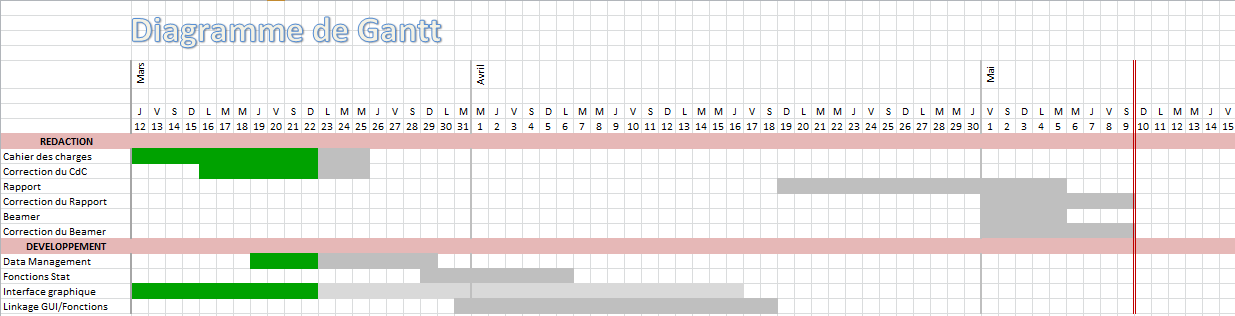
\includegraphics[width=15cm]{D_Gantt_II.png}
\end{center}

\subsection{Glossaire}
\begin{itemize}

\item{Framework : correspond à un ensemble de composants logiciels ayant le même paradigme, ce qui constitue un cadre de travail.} \\

\item{GUI : Graphical User Interface, c'est l'acronyme utilisé pour désigner l'interface graphique.}\\

\item{Benchmark : C'est un test de performance qui permet de mesurer les performances d'un système pour le comparer à d'autres systèmes.}\\

\item{ORM : Object-Role Modeling. Cela correspond à une technique pour représenter des données ainsi que leurs relations, sous forme d'objets. Cette méthode est généralement implémentées par trois pattern possibles : Table Data Gateway, Active Record, Data Access Object.}\\

\item{SGBDR : Systeme de Gestion de Base de Données Relationnelle.}\\

\item{SQL : Structured Query Language, désigne un langage de requête structurée servant à exploiter des bases de données relationnelles.}\\

\item{UDF: User-defined functions, fonction définies par les utilisateurs}\\

\item{DBA, pour DataBase Administrator est un Administrateur de base de données.} \\

\item{Binding de langage : permet l'utilisation d'une bibliothèque logicielle dans un autre langage de programmation que celui avec lequel elle a été écrite.}


\end{itemize}

\bibliographystyle{ieeetr}
\bibliography{CDC}

\end{document}